\section{Data Release Production}
\label{sec:drp}

\begin{figure}
\centering
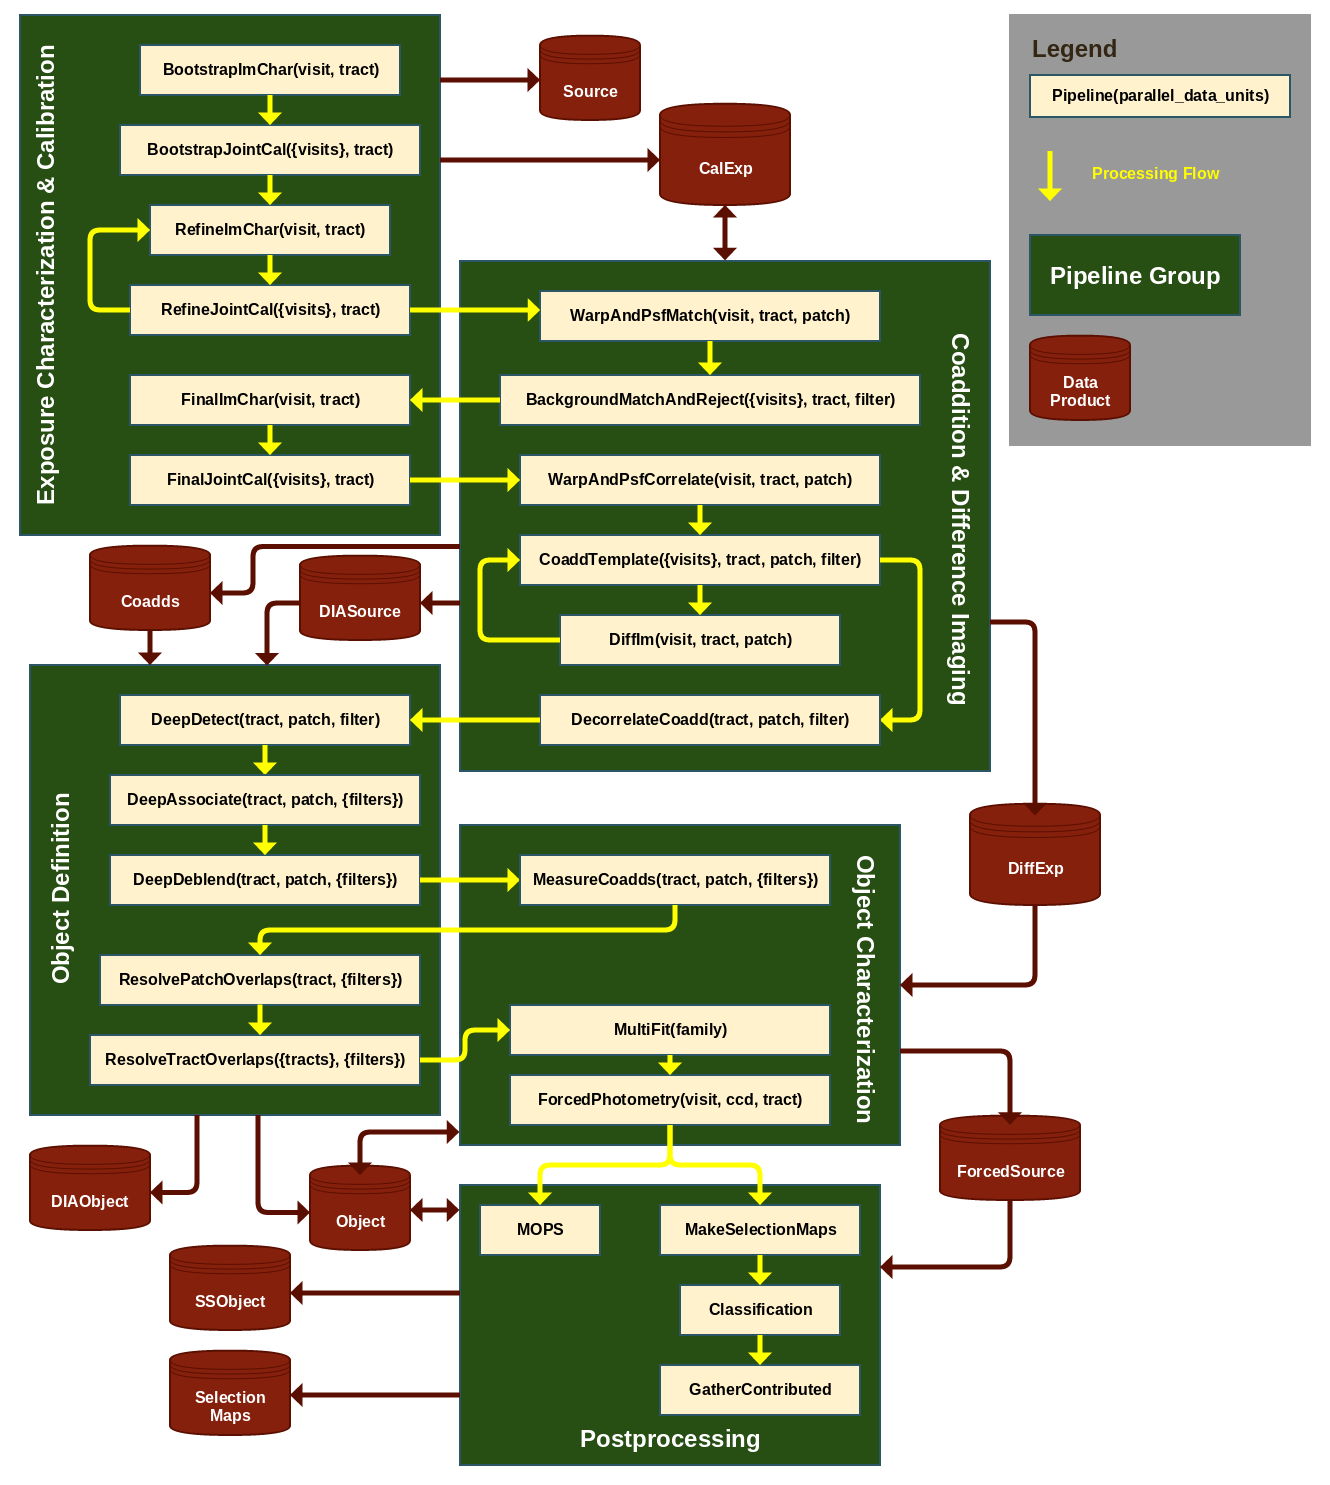
\includegraphics[width=\textwidth]{figures/drp_summary.png}
\caption{Summary of the Data Release Production processing flow.  Processing is split into multiple pipelines, which are conceptually organized into the groups discussed in sections~\ref{sec:drp_imchar_and_jointcal}-\ref{sec:drp_postprocessing}.
\label{fig:drp_summary}}
\end{figure}

\begin{note}[TODO]
  Update figure to reflect changes to sections in text.
\end{note}

A Data Release Production is run every year (twice in the first year of operations) to produce a set of catalog and image data products derived from all observations from the beginning of the survey to the point the production began.  This includes running a variant of the difference image analysis run in Alert Production, in addition to direct analysis of individual exposures and coadded images.  The data products produced by a Data Release Production are summarized in table~\ref{table:drp_data_products}.


\begin{table}
\small
\begin{tabularx}{\textwidth}{ | l | l | X | }
  \hline
  {\bf Name} & {\bf Availability} & {\bf Description} \\
  \hline
  Source & Stored &
  Measurements from direct analysis of individual exposures. \\
  \hline
  DIASource & Stored &
  Measurements from difference imagine analysis of individual exposures. \\
  \hline
  Object & Stored &
  Measurements for a single astrophysical object, derived from all available information, including coadd measurements, simultaneous multi-epoch fitting, and forced photometry.  Does not include solar system objects. \\
  \hline
  DIAObject& Stored &
  Aggregate quantities computing by associating spatially colocated DIASources. \\
  \hline
  ForcedSource & Stored &
  Flux measurements on each direct and difference image at the position of every Object. \\
  \hline
  SSObject & Stored &
  Solar system objects derived by associating DIASources and inferring their orbits. \\
  \hline
  CalExp & Regenerated &
  Calibrated exposure images for each CCD/visit (sum of two snaps). \\
  \hline
  DiffExp & Regenerated &
  Difference between CalExp and PSF-matched template coadd. \\
  \hline
  DeepCoadd & Stored &
  Coadd image with a reasonable combination of depth and resolution. \\
  \hline
  EpochRangeCoadd & Renegerated &
  Coadd image that cover only a limited range of epochs. \\
  \hline
  BestSeeingCoadd & Regenerated &
  Coadd image built from only the best-seeing images. \\
  \hline
  PSFMatchedCoadd & Regenerated &
  Coadd image with a constant, predetermined PSF. \\
  \hline
\end{tabularx}
\caption{Table of public data products produced during a Data Release Production.  A full description of these data products can be found in the Data Products Definition Document (LSE-163).
\label{table:drp_data_products}}
\end{table}

From a conceptual standpoint, data release production can be split into five groups of pipelines, executed in approximately the following order:
\begin{enumerate}
\item We characterize and calibrate each exposure, estimating point-spread functions, background models, and astrometric and photometric calibration solutions.  This iterates between processing individual exposures independently and jointly fitting catalogs derived from multiple overlapping exposures.  These steps are described more fully in section~\ref{sec:drp_imchar_and_jointcal}.
\item We alternately combine images and subtract them, using differences to find artifacts and time-variable sources while building coadds that produce a deeper view of the static sky.  Coaddition and difference imaging is described in section~\ref{sec:drp_coaddition_and_diffim}.
\item After all image processing is complete, we run additional catalog-only pipelines to fill in additional object properties.  Unlike previous stages, this postprocessing is not localized on the sky, as it may use statistics computed from the full data release to improve our characterization of individual objects.  Postprocessing pipelines are described in section~\ref{sec:drp_postprocessing}.
\end{enumerate}
This conceptual ordering is an oversimplification of the actual processing flow, however; as shown in Figure~\ref{fig:drp_summary}, pipeline groups are actually interleaved.

Each pipeline in this the diagram represents a particular piece of code excuted in parallel on a specific unit of data, but pipelines may contain additional (and more complex) parallelization to further subdivide that data unit.  The processing flow also includes the possibility of iteration between pipelines, indicated by cycles in the diagram.  The number of iterations in each cycle will be determined (via tests on smaller productions) before the start of the production, allowing us to remove these cycles simply by duplicating some pipelines a fixed number of times.  The final data release production processing can thus be described as a directed acyclic graph (DAG) to be executed by the orchestration middleware, with pipelines as edges and (intermediate) data products as vertices.  Most of the graph will be generated by applications code before the production begins, using a format and/or API defined by the orchestration middleware.  Howver, some parts of the graph must be generated on-the-fly; this will be discussed further in section~\ref{sec:drpMultiFit}.


\subsection{Image Characterization and Calibration}
\label{sec:drp_imchar_and_jointcal}

\begin{note}[ImChar/JointCal Diagram]
Extract ImChar/JointCal pipelines from ``DRP Top-Level Overview'' on confluence and expand detail to show data flow and ordering of ``Task/Process'' boxes.
\end{note}

The first steps in a Data Release Production characterize the properties of individual exposures, by iterating between pixel-level processing of individual visits (``ImChar'', or ``Image Characterization'' steps) and joint fitting of all catalogs overlapping a tract (``JointCal'', or ``Joint Calibration'' steps).  All ImChar steps involve fitting the PSF model and measuring Sources (gradually improving these as we iterate), while JointCal steps fit for new astrometric (WCS) and photometric solutions while building new reference catalogs for the ImChar steps.  Iteration is necessary for a few reasons:
\begin{itemize}
\item The PSF and WCS must have a consistent definition of object centroids.  Celestial positions from a reference catalog are transformed via the WCS to set the positions of stars used to build the PSF model, but the PSF model is then used to measure debiased centroids that feed the WCS fitting.
\item The later stages of photometric calibration and PSF modeling require secure star selection and colors to infer their SEDs.  Magnitude and morphological measurements from ImChar stages are aggregated the reference catalog in the subsequent JointCal stage, allowing these colors and classifications to be used for PSF modeling in the following ImChar stage.
\end{itemize}

The ImChar and JointCal iteration is itself interleaved with background matching and difference imaging, as described in section~\ref{sec:drp_coaddition_and_diffim}.  This allows the better backgrounds and masks to be defined by comparisons between images before the final Source measurements, image characterizations, and calibrations.

Each ImChar pipeline runs on a single visit, and each JointCal pipeline runs simultaneously on all visits within a single tract, allowing tracts to be run entirely independently.

The final output data products of the ImChar/JointCal iteration are the Source table and most of the CalExp (calibrated exposure) images.  CalExp is an \hyperref[sec:spImagesExposure]{Exposure}, and hence has Image, Mask, Variance, Background, PSF, WCS, and PhotoCalib components that we will track separately.

\subsubsection{BootstrapImChar}
\label{sec:drpBootstrapImChar}

The BootstrapImChar pipeline is the first thing run on each science exposure in a data release.  It has the difficult task of bootstrapping multiple quantities (PSF, WCS, photometric calibration, background model, etc.) that each normally require all of the others to be specified when one is fit.  As a result, while the algorithmic components to be run in this pipeline are generally clear, their ordering and specific requirements are not; algorithms that are run early will have a harder task than algorithms that are run later, and some iteration will almost certainly be necessary.

A plausible (but by no means certain) high-level algorithm for this pipeline is given below in pseudocode.  Highlighted terms are described in more detail below the pseudocode block.

\lstset{
    language=Python,
    basicstyle=\scriptsize\ttfamily,
    keywordstyle=\bfseries,
    commentstyle=\color{darkgray},
    escapeinside={\%}{\%},
}

% Define a local macro that lets us refer to sections of the text
% more easily (will undefine at the end of this section).
\newcommand{\hr}[1]{\hyperref[sec:drpBootstrapImChar_#1]{#1}}

\begin{lstlisting}
def BootstrapImChar(%\hr{raw}%, %\hr{reference}%):
    # Some data products components are visit-wide and some are per-CCD;
    # these imaginary data types lets us deal with both.
    # VisitExposure also has components; most are self-explanatory, and
    # {mi} == {image,mask,variance} (for "MaskedImage").
    calexp = VisitExposure()
    sources = VisitCatalog()
    snaps = VisitMaskedImageList()  # holds both snaps, but only {image,mask,variance}
    parallel for ccd in ALL_SENSORS:
        snaps[ccd] = [%\hr{RunISR}%(raw[ccd]) for snap in SNAP_NUMBERS]
        snaps[ccd].mask = %\hr{SubtractSnaps}%(snaps[ccd])
        calexp[ccd].mi = %\hr{CombineSnaps}%(snaps[ccd])
    calexp.psf = %\hr{FitWavefront}%(calexp[WAVEFRONT_SENSORS].mi)
    calexp.{image,mask,variance,background}
        = %\hr{SubtractBackground}%(calexp.mi)
    parallel for ccd in ALL_SENSORS:
        sources[ccd] = %\hr{DetectSources}%(calexp.{mi,psf})
    sources[ccd] = %\hr{DeblendSources}%(sources[ccd], calexp.{mi,psf})
    sources[ccd] = %\hr{MeasureSources}%(sources[ccd], calexp.{mi,psf})
    matches = %\hr{MatchSemiBlind}%(sources, reference)
    while not converged:
        %\hr{SelectStars}%(matches, exposures)
        calexp.wcs = %\hr{FitWCS}%(matches, sources, reference)
        calexp.psf = %\hr{FitPSF}%(matches, sources, calexp.{mi,wcs})
        %\hr{WriteDiagnostics}%(snaps, calexp, sources)
        parallel for ccd in ALL_SENSORS:
            snaps[ccd] = %\hr{SubtractSnaps}%(snaps[ccd], calexp[ccd].psf)
            calexp[ccd].mi = %\hr{CombineSnaps}%(snaps[ccd])
            calexp[ccd].mi = %\hr{SubtractStars}%(calexp[ccd].{mi,psf}, sources[ccd])
        calexp.{mi,background} = %\hr{SubtractBackground}%(calexp.mi)
        parallel for ccd in ALL_SENSORS:
            sources[ccd] = %\hr{DetectSources}%(calexp.{mi,psf})
            calexp[ccd].mi, sources[ccd] =
                %\hr{ReinsertStars}%(calexp[ccd].{mi,psf}, sources[ccd])
            sources[ccd] = %\hr{DeblendSources}%(sources[ccd], calexp.{mi,psf})
            sources[ccd] = %\hr{MeasureSources}%(sources[ccd], calexp.{mi,psf})
        matches = %\hr{MatchNonBlind}%(sources, reference)
    calexp.psf.apcorr = %\hr{FitApCorr}%(matches, sources)
    parallel for ccd in SCIENCE_SENSORS:
        sources[ccd] = %\hr{ApplyApCorr}%(sources[ccd], calexp.psf)
    return calexp, sources
\end{lstlisting}

\paragraph{Input Data Product: Raw}
\label{sec:drpBootstrapImChar_raw}

Raw amplifier images from science and wavefront CCDs, spread across one or more snaps.  Needed telescope telemetry (seeing estimate, approximate pointing) is assumed to be included in the raw image metadata.

\paragraph{Input Data Product: Reference}
\label{sec:drpBootstrapImChar_reference}

A full-sky catalog of reference stars derived from both external (e.g. Gaia) and LSST data.

The \hyperref[sec:drpStandardJointCal]{StandardJointCal} pipeline will later define a deeper reference catalog derived from this one and the new data being processed, but the origin and depth of the initial reference catalog is largely TBD.  It will almost certainly include Gaia stars, but it may also include data from other telescopes, LSST special programs, LSST commissioning observations, and/or the last LSST data release.  Decisions will require some combination of negotation with the LSST commissioning team, specification of the special programs, quality analysis and experimentation with the Gaia catalog, and policy decisions from DM leadership on the degree to which data releases are required to be independent.  Depending on the choices selected, it could also require a major separate processing effort using modified versions of the data release production pipelines.

\paragraph{Output Data Product: Source}
\label{sec:drpBootstrapImChar_sources}

A preliminary version of the Source table.  This could contain all of the columns in the DPDD Source schema if the \hr{MeasureSources} is appropriately configured, but some of these columns are likely unnecessary in its role as an intermediate data product that feeds \hyperref[sec:drpStandardJointCal]{StandardJointCal}, and it is likely that other non-DPDD columns will be present for that role.

BootstrapImChar also has the capability to produce even earlier versions of the Source table for diagnostic purposes (see \hr{WriteDiagnostics}).  These tables are not associated with any photometric calibration or aperture correction, and some may not have any measurements besides centroids, and hence are never substitutable for the final Source table.

\paragraph{Output Data Product: CalExp}
\label{sec:drpBootstrapImChar_calexp}

A preliminary version of the CalExp (calibrated direct exposure).  CalExp is an \hyperref[sec:spImagesExposure]{Exposure} object, and hence it has several components.  BootstrapImChar is the only pipeline that actually updates all of them.  Some CalExp components are determined at the scale of a full FoV and hence should probably be persisted at the visit level (PSF, WCS, PhotoCalib, Background), while others are straightforward CCD-level data products (Image, Mask, Variance).

\paragraph{RunISR}
\label{sec:drpBootstrapImChar_RunISR}

Delegate to the \hyperref[sec:acISR]{ISR algorithmic component} to perform standard detrending as well as brighter-fatter correction and interpolation for pixel-area variations (\hyperref[sec:acFixPixelAreaVariations]{Warping Irregularly-Sampled Images}).  It is possible that these corrections will require a PSF model, and hence must be backed-out and recorrected at a later stage when an improved PSF model is available.

We assume that the applied flat field is appropriate for background estimation.

\paragraph{SubtractSnaps}
\label{sec:drpBootstrapImChar_SubtractSnaps}

Delegate to the \hyperref[sec:acSnapSubtraction]{Snap Subtraction algorithmic component} to mask artifacts in the difference between snaps.  If passed a PSF (as in the second call), also interpolate them by delegating to the \hyperref[sec:acArtifactInterpolation]{Artifact Interpolation} algorithmic component.

We assume here that the PSF modeled on the combination of the two Snaps is sufficient for interpolation on the Snaps individually; if this is not true, we can just mask and interpolate both Snaps when an artifact appears on either of them (or we could do per-Snap PSF estimation, but that's a lot more work for very little gain).

\paragraph{CombineSnaps}
\label{sec:drpBootstrapImChar_CombineSnaps}

Delegate to the \hyperref[sec:acCoaddition]{Image Coaddition algorithmic component} to combine the two Snaps while handling masks appropriately.

We assume there is no warping involved in combining snaps.  If this is needed, we should instead advocate for dropping snaps in favor of a a single longer exposure.

\paragraph{FitWavefront}
\label{sec:drpBootstrapImChar_FitWavefront}

Delegate to the \hyperref[sec:acWavefrontSensorPSF]{Wavefront Sensor PSF algorithmic component} to generate an approximate PSF using only data from the wavefront sensors and observational metadata (e.g. reported seeing).

Processing the wavefront sensors will likely require some form of detection and measurement; we currently consider this to be part of the \hyperref[sec:acWavefrontSensorPSF]{Wavefront Sensor PSF} code, though it may delegate to e.g. \hyperref[sec:acSourceDetection]{Source Detection} and/or \hyperref[sec:acSingleFrameMeasurement]{Single Frame Measurement}.

The required quality of this PSF estimate is TBD; setting preliminary requirements will involve running a version of BootstrapImChar with at least mature detection and PSF-modeling algorithms on precursor data taken in crowded fields, and final requirements will require proceessing full LSST camera data in crowded fields.  However, robustness to poor data quality and crowding is much more important than accuracy; this stage need only provide a good enough result for subsequent stages to prcoeed.

\paragraph{SubtractBackground}
\label{sec:drpBootstrapImChar_SubtractBackground}

Delegate to the \hyperref[sec:acBackgroundEstimation]{Background Estimation} algorithmic component to model and subtract the background consistently over the full field of view.

The multiple backgrounds subtracted in BootstrapImChar may or may not be cumulative (i.e. we may or may not add the previous background back in before estimating the latest one).

\paragraph{DetectSources}
\label{sec:drpBootstrapImChar_DetectSources}

Delegate to the \hyperref[sec:acSourceDetection]{Source Detection algorithmic component} to find above-threshold regions (\hyperref[sec:spFootprints]{Footprints}) and peaks within them in a PSF-correlated version of the image.

In crowded fields, each iteration of detection will decrease the threshold, increasing the number of objects detection.  Because this will treat fluctuations in the background due to undetected objects as noise, we may need to extend PSF-correlation to the appropriate filter for an image with correlated noise and characterize the noise field from the image itself.

Because we will use wavefront data to constrain the PSF, we also run detection on the wavefront sensors.  It is possible that this will require a different algorithmic component if we cannot just treat the wavefront sensors as science sensors with an out-of-focus PSF.

\paragraph{DeblendSources}
\label{sec:drpBootstrapImChar_DeblendSources}

Delegate to the \hyperref[sec:acSingleFrameDeblending]{Single Frame Deblending algorithmic component} to split \hyperref[sec:spFootprints]{Footprints} with multiple peaks into deblend families.

Because we will use wavefront data to constrain the PSF, we also run deblending on the wavefront sensors.  It is possible that this will require a different algorithmic component if we cannot just treat the wavefront sensors as science sensors with an out-of-focus PSF, and we need deblending to extract wavefront information.

\paragraph{MeasureSources}
\label{sec:drpBootstrapImChar_MeasureSources}

Delegate to the \hyperref[sec:acSingleFrameMeasurement]{Single Frame Measurement algorithmic component} to measure source properties.

In BootstrapImChar, we anticipate using the \hyperref[sec:acReplaceNeighborsWithNoise]{Neighbor Noise Replacement} approach to deblending, with the following plugin algorithms:
\begin{itemize}
\item \hyperref[sec:acCentroidAlgorithms]{Centroids}
\item \hyperref[sec:acShapeAlgorithms]{Second-Moment Shapes}
\item \hyperref[sec:acPixelFlags]{Pixel Flag Aggregation}
\item \hyperref[sec:acAperturePhotometry]{Aperture Photometry} (but only for one or two radii)
\item \hyperref[sec:acStaticPointSourceModels]{Static Point Source Models}
\end{itemize}

Because we will use wavefront data to constrain the PSF, we also run measurement on the wavefront sensors (but probably without any flux measurement algorithms, and perhaps with modified versions of other algorithms).  It is possible that this will require a different algorithmic component if we cannot just treat the wavefront sensors as science sensors with an out-of-focus PSF.

\paragraph{MatchSemiBlind}
\label{sec:drpBootstrapImChar_MatchSemiBlind}

Delegate to the \hyperref[sec:acSingleVisitReferenceMatching]{Single Visit Reference Matching algorithmic component} to match source catalogs to a global reference catalog.  This occurs over the full field of view, ensuring robust matching even when some CCDs have no matchable stars due to crowding, flux limits, or artifacts.

``Semi-Blind'' refers to the fact that the WCS is not yet well known (all we have is what is provided by the observatory), so the matching algorithm must account for an unknown (but small) offset between the WCS-predicted sources positions and the reference catalog positions.

\paragraph{SelectStars}
\label{sec:drpBootstrapImChar_SelectStars}

Use reference catalog classifications and source flags to select a clean sample stars to use for later stages.

If we decide not to rely on a pre-existing reference catalog to separate stars from galaxies and other objects, we will need a new algorithmic component to select stars based on source measurements.

\paragraph{FitWCS}
\label{sec:drpBootstrapImChar_FitWCS}

Delegate to the \hyperref[sec:acSingleVisitAstrometricFit]{Single Visit Astrometric Fit algorithmic component} to determine the WCS of the image.

We assume this works by fitting a simple mapping from the visit's focal plane coordinate system to the sky and composing it with the (presumed fixed) mapping between CCD coordinates and focal plane coordinates.  This fit will be improved in later pipelines, so it does not need to be exact; $<$0.05 arcsecond accuracy should be sufficient.

As we iterate in crowded fields, the number of degrees of freedom in the WCS should be allowed to slowly increase.

\paragraph{FitPSF}
\label{sec:drpBootstrapImChar_FitPSF}

Delegate to the \hyperref[sec:acFullVisitPSF]{Full Visit PSF Modeling algorithmic component} to construct an improved PSF model for the image.

Because we are relying on a reference catalog to select stars, we should be able to use colors from the reference catalog to estimate SEDs an include wavelength dependence in the fit.  If we do not use a the reference catalog early in BootstrapImChar, PSF estimation here will not be wavelength-dependent.  In either case the PSF model will be further improved in later pipelines.

PSF estimation at this stage must include some effort to model the wings of bright stars, even if this is tracked and constrained separately from the model for the core of the PSF.

As we iterate in crowded fields, the number of degrees of freedom in the PSF model should be allowed to slowly increase.

\paragraph{WriteDiagnostics}
\label{sec:drpBootstrapImChar_WriteDiagnostics}

If desired, the current state of the \texttt{source}, \texttt{calexp}, and \texttt{snaps} variables may be persisted here for diagnostic purposes.

\paragraph{SubtractStars}
\label{sec:drpBootstrapImChar_SubtractStars}

Subtract all detected stars above a flux limit from the image, using the PSF model.  In crowded fields, this should allow subsequent \hr{SubtractBackground} and \hr{DetectSources} steps to push fainter by removing the brightest stars in the image.

Sources classified as extended are never subtracted.

\paragraph{ReinsertStars}
\label{sec:drpBootstrapImChar_ReinsertStars}

Add stars removed in \hr{SubtractStars} back into the image, and merge corresponding \hyperref[sec:spFootprints]{Footprints} and peaks into the source catalog.

\paragraph{MatchNonBlind}
\label{sec:drpBootstrapImChar_MatchNonBlind}

Match a single-CCD source catalog to a global reference frame, probably by delegating to \hyperref[sec:acJointCalMatching]{the same matching algorithm used in JointCal pipelines}.  A separate algorithm component may be needed for efficiency or code maintenance reasons; this is a simple limiting case of the multi-way JointCal matching problem that may or may not merit a separate simpler implementation.

``Non-Blind'' refers to the fact that the WCS is now known well enough that there is no significant offset between WCS-projected source positions and reference catalog positions.

\paragraph{FitApCorr}
\label{sec:drpBootstrapImChar_FitApCorr}

Delegate to the \hyperref[sec:acApCorr]{Aperture Correction algorithmic component} to construct a curve of growth from aperture photometry measurements and build an interpolated mapping from other fluxes to the predicted integrated flux at infinity.

\paragraph{ApplyApCorr}
\label{sec:drpBootstrapImChar_ApplyApCorr}

Delegate to the \hyperref[sec:acApCorr]{Aperture Correction algorithmic component} to apply aperture corrections to flux measurements.

% Undeclare the local hyperref macro
\let\hr\undefined

\subsubsection{StandardJointCal}
\label{sec:drpStandardJointCal}

In StandardJointCal, we jointly process all of the Source tables produced by running \hyperref[sec:drpBootstrapImChar]{BootstrapImChar} on each visit in a tract.  There are four steps:
\begin{enumerate}
\item We match all sources and the reference catalog by delegating to \hyperref[sec:acJointCalMatching]{JointCalMatching}.  This is a non-blind search; we assume the WCSs output by \hyperref[sec:drpBootstrapImChar]{BootstrapImChar} are good enough that we don't need to fit for any additional offsets between images at this stage.  Some matches will not include a reference object, as the sources will almost certainly extend deeper than the reference catalog.
\item We classify matches to select a clean sample of low-variability stars for later steps, delegating to \hyperref[sec:acJointCalClassification]{JointCalClassification}.  This uses morphological and possibly color information from source measurements as well as reference catalog information (where available).  This step also assigns an inferred SED to each match from its colors; for matches associated with a reference object, whether this supersedes SEDs or colors in the reference catalog is depends on our approach to absolute calibration.
\item We fit simultaneously for improved astrometric solution by requiring each star in a match to have the same position.  This may need to correct (perhaps approximately) for centroid shifts due to DCR and/or proper motion; if it does not, it must be robust against these shifts (perhaps via outlier rejection).  The models and parameters to fit must be determined by experimentation, but they will represent further perturbation of the WCS fit in BootstrapImChar.  This fit generates a new WCS component for each CalExp.
\item We fit simultaneously for photometric zeropoints by requiring each star in a match to have the same flux after applying smoothed monochromatic flat fields produced by the calibration products pipeline.  There is a small chance this fit will also be used to further constrain those monochromatic flat fields.  This fit generates a new PhotoCalib component for each CalExp.
\end{enumerate}

In addition to updating the CalExp WCS and PhotoCalib, StandardJointCal generates a new Reference dataset containing the joint-fit centroids and fluxes for each of its match groups as well as their classifications and inferred SEDs.

StandardJointCal may be iterated with \hyperref[sec:drpRefineImChar]{RefineImChar} to ensure the PSF and WCS converge on the same centroid definitions.  StandardJointCal is always run immediately after \hyperref[sec:drpBootstrapImChar]{BootstrapImChar}, but \hyperref[sec:drpRefineImChar]{RefineImChar} or \hyperref[sec:drpStandardJointCal]{StandardJointCal} may be the last step in the iteration run before proceding with \hyperref[sec:drpWarpAndPsfMatch]{WarpAndPsfMatch}.

\subsubsection{RefineImChar}
\label{sec:drpRefineImChar}

RefineImChar performs an incremental improvement on the measurements and PSF model produced by \hyperref[sec:drpBootstrapImChar]{BootstrapImChar}, using the improved reference catalog, WCS, and PhotoCalib produced by \hyperref[sec:drpStandardJointCal]{StandardJointCal}.  Its steps are thus a strict subset of those in \hyperref[sec:drpBootstrapImChar]{BootstrapImChar}.  A pseudocode description of RefineImChar is given below, but all steps refer to back to the descriptions in \ref{sec:drpBootstrapImChar}:

% Redefine the BootstrapImChar macro, since we'll refer back to those
% sections here.
\newcommand{\hr}[1]{\hyperref[sec:drpBootstrapImChar_#1]{#1}}

\begin{lstlisting}
def RefineImChar(%\hr{calexp}%, %\hr{sources}%, %\hr{reference}%):
    matches = %\hr{MatchNonBlind}%(sources, reference)
    %\hr{SelectStars}%(matches, exposures)
    calexp.psf = %\hr{FitPSF}%(matches, sources, calexp.{mi,wcs})
    parallel for ccd in ALL_SENSORS:
        calexp[ccd].mi = %\hr{SubtractStars}%(calexp[ccd].{mi,psf}, sources[ccd])
    calexp.{mi,background} = %\hr{SubtractBackground}%(calexp.mi)
    parallel for ccd in ALL_SENSORS:
        sources[ccd] = %\hr{DetectSources}%(calexp.{mi,psf})
        calexp[ccd].mi, sources[ccd] =
            %\hr{ReinsertStars}%(calexp[ccd].{mi,psf}, sources[ccd])
        sources[ccd] = %\hr{DeblendSources}%(sources[ccd], calexp.{mi,psf})
        sources[ccd] = %\hr{MeasureSources}%(sources[ccd], calexp.{mi,psf})
    calexp.psf.apcorr = %\hr{FitApCorr}%(matches, sources)
    parallel for ccd in ALL_SENSORS:
        sources[ccd] = %\hr{ApplyApCorr}%(sources[ccd], calexp.psf)
    return calexp, sources
\end{lstlisting}

This is essentially just another iteration of the loop in in \hyperref[sec:drpBootstrapImChar]{BootstrapImChar}, without the WCS-fitting or artifact-handling stages.  We assume that we continue to process the wavefront sensors here (because we will use them in the \hr{FitPSF} step), but it may be that previous processing may be sufficient.

Note that RefineImChar does not update the CalExp's WCS, PhotoCalib, Image, or Variance (and its Mask is only updated to indicate new detections).


% Undeclare the local hyperref macro
\let\hr\undefined

\subsubsection{FinalImChar}
\label{sec:drpFinalImChar}

FinalImChar is responsible for producting the final PSF models and source measurements.  While similar to \hyperref[sec:drpRefineImChar]{RefineImChar}, it is run after at least one iteration of the \hyperref[sec:drpBackgroundMatchAndReject]{BackgroundMatchAndReject} and possibly \hyperref[sec:drpUpdateMasks]{UpdateMasks} pipelines, which provide it with the final background model and mask.

The steps in FinalImChar are identical to those in \hyperref[sec:drpRefineImChar]{RefineImChar}, with just a few exceptions:

\begin{itemize}
\item The background is not re-estimated and subtracted.
\item The suite of plugin run by \hyperref[sec:acSingleFrameMeasurement]{Single Frame Measurement} is expanded to included all algorithms indicated in the first column of Figure~\ref{fig:measurement-matrix}.  This should provide all measurements in the DPDD Source table description.
\item We also classify sources by delegating to \hyperref[sec:acSingleFrameClassification]{Single Frame Classification}, to fill the final Source table's \emph{extendedness} field.  It is possible this will also be run during \hyperref[sec:drpRefineImChar]{RefineImChar} and \hyperref[sec:drpBootstrapImChar]{BootstrapImChar} for diagnostic purposes.
\end{itemize}

\subsubsection{FinalJointCal}
\label{sec:drpFinalJointCal}

FinalJointCal is \emph{almost} identical to \hyperref[sec:drpStandardJointCal]{StandardJointCal}, and the details of the differences when surrounding pipelines are more mature and the approach to absolute calibration is more clear.  Because it is responsible for the final photometric calibration, it may be need to perform some steps that could be omitted from \hyperref[sec:drpStandardJointCal]{StandardJointCal} because they have no impact on the ImChar pipelines.  This could include a role in determining the absolute photometric calibration of the survey, especially if an external catalog (e.g. Gaia) is relied upon exclusively to tie different tracts together.

There is no need for FinalJointCal to produce a new or updated Reference dataset (except for its own internal use), as subsequent steps do not need one, and the DRP-generated reference catalog used by Alert Production will be derived from the Object table.

Unlike \hyperref[sec:drpStandardJointCal]{StandardJointCal}, FinalJointCal is also responsible for applying its improved photometric and astrometric calibrations to raw the Source table generated by \hyperref[sec:drpFinalImChar]{FinalImChar}, yielding a Source table suitable for database ingest.  However, if the final \emph{absolute} calibration is not determined by FinalJointCal, these will need to be further adjusted at a later stage (probably after database ingest).

\subsection{Coaddition and Difference Imaging}
\label{sec:drp_coaddition_and_diffim}

The next group of pipelines in a Data Release Production consist of image coaddition and image differencing, which we use to separate the static sky from the dynamic sky in terms of both astrophysical quantities and observational quantities.  This group also includes an iteration between pipelines that combine images and pipelines that subtract the combined images from each exposure.  At each differencing step, we better characterize the features that are unique to a single epoch (whether artifacts, background features, or astrophysical sources); we use these characterizations to ensure the next round of coadds include only features that are common to all epochs.

\begin{figure}
\centering
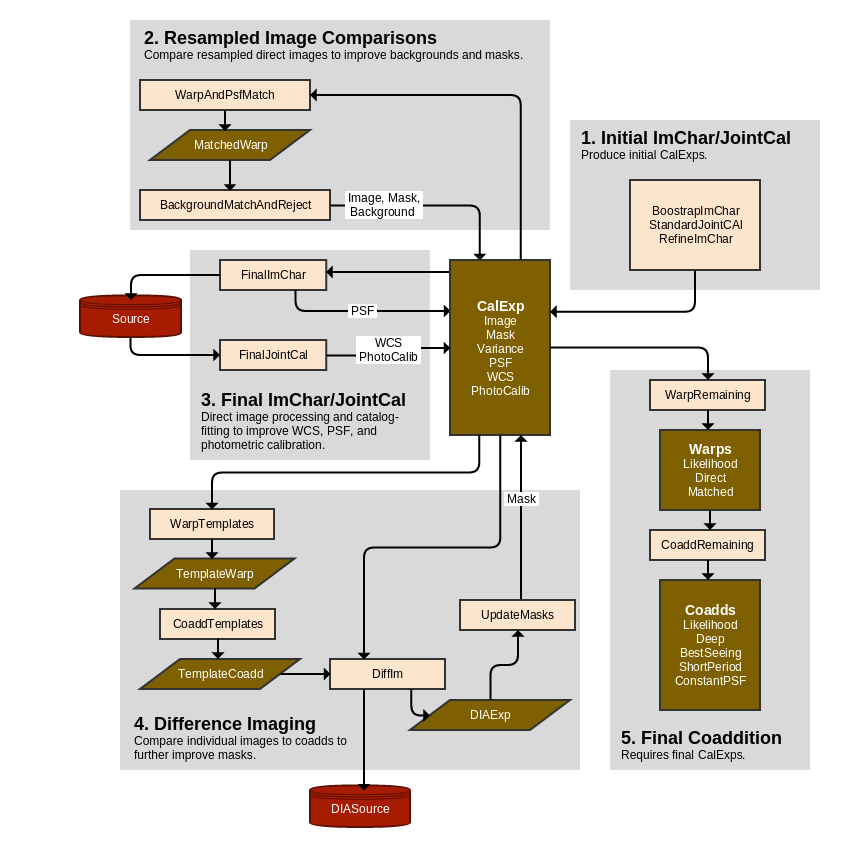
\includegraphics[width=\textwidth]{figures/drp_coaddition_and_diffim.png}
\caption{
  Data flow diagram for the Data Release Production coaddition and difference imaging pipelines.  Processing proceeds roughly counterclockwise, starting from the upper right with pipelines described in Section~\ref{sec:drp_imchar_and_jointcal}.  Each update to a component of the central CalExp dataset can in theory trigger another iteration of a previous loop, but in practice we will ``unroll'' these loops before production begins, yielding an acyclic graph with a series of incrementally updated CalExp datasets.  The nature of this unrolling and the number of iterations will be determined by future algorithmic research.  Numbered steps above are described more fully in the text.
  \label{fig:drp_coaddition_and_diffim}
}
\end{figure}

The processing flow in this pipeline group again centers around incremental updates to the CalExp dataset, which are limited here to its Background and Mask component (the Image component is also updated, but only to subract the updated background).  It will also return to the previous pipeline group described in Section~\ref{sec:drp_imchar_and_jointcal} to update other CalExp components.  The data flow between pipelines is shown in Figure~\ref{fig:drp_coaddition_and_diffim}, with the numbered steps are described further below:
\begin{enumerate} % note that the figure numbers aren't automatically linked
\item The first version of the CalExp dataset is produced by running the \hyperref[sec:drpBootstrapImChar]{BootstrapImChar}, \hyperref[sec:drpStandardJointCal]{StandardJointCal}, and \hyperref[sec:drpRefineImChar]{RefineImChar} pipelines, as described in Section~\ref{sec:drp_imchar_and_jointcal}.
\item We generate an updated Background and Mask via the \hyperref[sec:drpWarpAndPsfMatch]{WarpAndPsfMatch} and \hyperref[sec:drpBackgroundMatchAndReject]{BackgroundMatchAndReject} pipelines.  This produces the final CalExp Background and Image, and possibly the final Mask.
\item If the CalExp Mask has been finalized, we run the \hyperref[sec:drpFinalImChar]{FinalImChar} and \hyperref[sec:drpFinalJointCal]{FinalJointCal} pipelines.  These produce the final PSF, WCS, and PhotoCal.  If the Mask has not been finalized, we execute at least one iteration of the next step before this one.
\item We run the \hyperref[sec:drpWarpTemplates]{WarpTemplates}, \hyperref[sec:drpCoaddTemplates]{CoaddTemplates}, and \hyperref[sec:drpDiffIm]{DiffIm} pipelines to generate the DIASource and DIAExp datasets.  We may then be able to generate better CalExp Masks than we can obtain from \hyperref[sec:drpBackgroundMatchAndReject]{BackgroundMatchAndReject} by comparing the DIAExp masks across visits in the \hyperref[sec:drpUpdateMasks]{UpdateMasks} pipeline.
\item After all CalExp components have been finalized, we run the \hyperref[sec:drpWarpRemaining]{WarpRemaining} and \hyperref[sec:drpCoaddRemaining]{CoaddRemaining} to build additional coadd data products.
\end{enumerate}
The baseline ordering of these steps is thus \{1,2,3,4,5\}, but \{1,2,4,3,4,5\} is perhaps just as likely, and we may ultimately require an ordering that repeats steps 2 or 3.  Final decisions on the ordering and number of iteration will require testing with mature pipelines and a deep dataset taken with a realistic cadence; it is possible the configuration could even change between data releases as the survey increases in depth.  Fortunately, this reconfiguring should not require significant new algorithm development.

This pipeline group is responsible for producing the following final data products:
\begin{description}
\item[CalExp.\{Image,Background,Mask\}]  See above.
\item[DIAExp] A CCD-level \hyperref[sec:spImagesExposure]{Exposure} that is the difference between the CalExp and a template coadd, in the coordinate system and with the PSF of the CalExp.
\item[DIASource] A \hyperref[sec:spTablesSource]{SourceCatalog} containing sources detected and measured on the DIAExp images.
\item[ConstantPSFCoadd] A coadd data product (\hyperref[sec:spImagesExposure]{Exposure} or subclass thereof) with a constant, predefined PSF.
\item[DeepCoadd] A coadd data product built to optimize depth at the possible expense of seeing.
\item[BestSeeingCoadd] A coadd data product built to optimize image quality at the possible expense of depth.  Depending on the algorithm used, this may be the same as DeepCoadd.
\item[ShortPeriodCoadd] A coadd data product built from exposures in a short range of epochs, such as a year, rather than the full survey.
\item[LikelihoodCoadd] A coadd formed by correlating each image with its own PSF before combining them, used for detection and possibly building other coadds.
\item[ShortPeriodLikelihoodCoadd] Short-period likelihood coadds will also be built.
\item[TemplateCoadd] A coadd data product used for difference imaging in both DRP and AP, \emph{or} some other tract/patch/filter data product from which the template for a given airmass can be derived.
\end{description}

The nature of these coadd data products depends critically on whether we are able to develop efficient algorithms for optimal coaddition, and whether these coadds are suitable for difference imaging.  These algorithms are mathematically well-defined but computationally difficult; see \href{http://dmtn-015.lsst.io/en/latest/}{DMTN-15} for more information.  We will refer to the coadds produced by these algorithms as ``decorrelated coadds''; a variant with constant PSF (``constant-PSF partially decorrelated coadd'') is also possible.  This choice is also mixed with the question of how we will correct for differential chromatic refraction in difference imaging; some algorithms for DCR correction involve templates that are the result of inference on input exposures rather than coaddition.  There are five main scenarios for our use of decorrelated coadds:
\begin{description}
  \item[A] We use decorrelated coadds for all final coadd products.  DeepCoadd and ShortPeriodCoadd will be standard decorrelated coadds with a spatially-varying PSF, and ConstantPSFCoadd and TemplateCoadd will be constant-PSF partially-decorrelated coadds.  The BestSeeingCoadd data product will be dropped, as it will be redundant with DeepCoadd.  This will make coadds more expensive and complex to build, and require more algorithm development for coaddition, but will improve coadd-based measurements and make it easier to warm-start multi-epoch measurements.  Difference imaging may be easier, and more visits may be usable as inputs to templates due to softened or eliminated seeing cut.
  \item[B] We use decorrelated coadds for all coadds but TemplateCoadd.  Measurement is still improved, and the additional computational cost of coaddition is limited to a single pipeline that is not run iteratively.  Difference imaging may be harder, and the number of visits eligible for inclusion in templates may be reduced.  In this scenario, we still have two options for building templates:
  \begin{description}
    \item[B1] Templates will be built as PSF-matched coadds, or a product of PSF-matched coadds.
    \item[B2] Templates are the result of inference on resampled exposures with no PSF-matching.
  \end{description}
  \item[C] We do not use decorrelated coadds at all.  DeepCoadd, BestSeeingCoadd, and ShortPeriodCoadd will be direct coadds, and ConstantPSFCoadd will be a PSF-matched coadd.  Coaddition will be simpler and faster, but downstream algorithms may require more sophistication, coadd measurements may be lower quality, and multi-epoch measurements may be more difficult to optimize.  Here we again have the same two options for templates as option \textbf{B}:
  \begin{description}
    \item[C1] Templates will be built as PSF-matched coadds, or a product of PSF-matched coadds.
    \item[C2] Templates are the result of inference on resampled exposures with no PSF-matching.
  \end{description}
\end{description}
It is also possible to combine multiple scenarios across different bands.  In particular, we may not need special templates to handle DCR in redder bands, so we may select a simpler approach to dealing with them in those bands.  The final selection between these options will require experiments on LSST data or precursor data with similar DCR and seeing, though decorrelated coaddition algorithms and some approaches to DCR correction may be ruled out earlier if preliminary algorithm development does not go well.

Further differences in the pipelines themselves due to the presence or absence of decorrelated coadds will be described in the sections below.

\subsubsection{WarpAndPsfMatch}
\label{sec:drpWarpAndPsfMatch}

This pipeline resamples and then PSF-matches CalExp images from a visit into a single patch-level image with a constant PSF.  The resampling and PSF-matching can probably be accomplished separately by delegating to the \hyperref[sec:acWarping]{Image Warping} and \hyperref[sec:acPSFHomogenization]{PSF Homogenization} algorithmic components, respectively.  These operations can also be performed in the opposite order if the matched-to PSF is first transformed to the CalExp coordinate systems (so subsequent resampling yields a constant PSF in the coadd coordinate system).  Doing PSF-matching first may be necessary (or at least easier to implement) for undersampled images.

It is possible these operations will be performed simultaneously by a new algorithmic component; this could potentially yield improved computational performance and make it easier to properly track uncertainty.  These improvements are unlikely to be necessary for this pipeline, because these images and the coadds we build from them will only be used to estimate backgrounds and find artifacts, and these operations only require approximate handling of uncertainty.  However, other coaddition pipelines may require building an algorithmic component capable of warping and PSF-matching simultaneously, and if that happens, we would likely use it here as well.

The only output of the WarpAndPsfMatch pipeline is the MatchedWarp \hyperref[sec:spImagesExposure]{Exposure} intermediate data product.  It contains all of the usual \hyperref[sec:spImagesExposure]{Exposure} components, which must be propagated through the image operations as well.  There is a separate MatchedWarp for each \{patch, visit\} combination, and these can be produced by running WarpAndPsfMatch independently on each such combination.  However, individual CCD-level CalExps will be required by multiple patches, so I/O use or data transfer may be improved by running all WarpAndPsfMatch instances for a given visit together.

\subsubsection{BackgroundMatchAndReject}
\label{sec:drpBackgroundMatchAndReject}

This pipeline is responsible for generating our final estimates of the sky background and updating our artifact masks.  It is one of the most algorithmically uncertain algorithms in Data Release Production, particularly from the standpoint of large-scale data flow and parallelization, because while the algorithm is well-defined and understood for a small patch of sky, we do not yet have a concrete approach for extending it to large fields containing multiple dithered images (though it has been demonstrated on SDSS data, for which the drift-scan observation strategy makes the problem simpler).  It still processes tracts independently, but below that scale the parallelization is very much uncertain, and may in fact involve splitting these operations further into smaller pipelines.

The steps involved in background matching are described below.  All of these operations are performed on the MatchedWarp images; these are all in the same coordinate system and have the same PSF, so they can be meaningfully added and subtracted with no additional processing.
\begin{enumerate}
\item We define one of the visits that overlap an area of the sky as the \emph{reference image}.  At least in the naive local specification of the algorithm, this image must be smooth and continous over the region of interest.  This is done by the \hyperref[sec:acBuildBackgroundReference]{Build Background Reference} pipeline, which must artificially (but reversibly) enforce continuity in a reference image that stitches together multiple visits to form a single-epoch-deep full tract image, unless we develop an approach for dealing with discontinuity downstream.
\item We subtract the reference image from every other visit image.  This must account for any artifical features due to the construction of the reference image.
\item We run \hyperref[sec:acSourceDetection]{Source Detection} on the per-visit difference images to find artifacts and transient sources.  We do not generate a traditional catalog of these detections, as they will only be used to generate improved CalExp masks; they will likely be stored as a sequence of \hyperref[sec:spFootprints]{Footprints}.
\item We estimate the background on the per-visit difference images by delegating to the \hyperref[sec:acBackgroundEstimation]{Background Estimation} algorithmic component.  This difference background should be easier to be model than a direct image background, as the image will be mostly free of sources and astrophysical backgrounds.
\item We build a PSF-matched coadd by adding all of the visit images (including the reference) and subtracting all of the difference image backgrounds; this yields a coadd that contains only the reference image background, which we then model and subtract by again using the \hyperref[sec:acBackgroundEstimation]{Background Estimation} algorithmic component.  Combining the images will be performed by the \hyperref[sec:acCoaddition]{Coaddition} algorithmic component, which will also generate new CalExp masks by analyzing the per-pixel, multi-visit histograms of image and mask values (e.g. generalized statistical outlier rejection) to distinguish transients and artifacts from variable sources.
\end{enumerate}

We are assuming in the baseline plan that we can use a matched-to PSF in \hyperref[sec:drpWarpAndPsfMatch]{WarpAndPsfMatch} large enough to match all visit images to it without deconvolution.  If a large marged-to PSF adversely affects subsequent processing in \hyperref[sec:drpBackgroundMatchAndReject]{BackgroundMatchAndReject}, we may need to develop an iterative approach in which we apply \hyperref[sec:drpWarpAndPsfMatch]{WarpAndPsfMatch} only to better-seeing visits first, using a smaller target PSF, run \hyperref[sec:drpBackgroundMatchAndReject]{BackgroundMatchAndReject} on these, and then re-match everything to a larger target PSF and repeat with a larger set of input visits.  However, this problem would suggest that the \hyperref[sec:drpDiffIm]{DiffIm} and \hyperref[sec:drpUpdateMasks]{UpdateMasks} pipelines would be even better at finding artifacts, so a more likely mitigation strategy would be to simply defer final Mask generation to after at least one iteration of those pipelines, as described in the discussion of Figure~\ref{fig:drp_coaddition_and_diffim} at the beginning of Section~\ref{sec:drp_coaddition_and_diffim}.

The outputs of BackgroundMarchAndReject are updated Background and Mask components for the CalExp product.  Because it is not built with the final photometric and astrometric calibration, the PSF-matched coadd built here is discarded.

\subsubsection{WarpTemplates}
\label{sec:drpWarpTemplates}

This pipeline is responsible for generating the resampled visit-level images (TemplateWarp) used to build template coadds for difference imaging.  The algorithmic content of this pipeline and the nature of its outputs depends on whether we are using decorrelated coadds (option \textbf{A}) at the beginning of \ref{sec:drp_coaddition_and_diffim}), PSF-matched coadds (\textbf{B1} or \textbf{C1}), or inferring templates (\textbf{B2} or \textbf{C2}).

If we are using decorrelated coadds (option \textbf{A}), the output is equivalent to the LikelihoodWarp data product produced by the \hyperref[sec:drpWarpRemaining]{WarpRemaining} pipeline (aside from differences due to the state of the input CalExps), and the algorithm to produce it the same:
\begin{itemize}
\item We correlate the image with its own PSF by delegating to the \hyperref[sec:spKernels]{Convolution Kernels} software primitive.
\item We resample the image by delegating to the \hyperref[sec:acWarping]{Image Warping} algorithmic component.
\end{itemize}
As with other convolution-and-warping pipelines, it is possible we will instead develop a single algorithmic component to perform both operations.  These operations must include full propogation of uncertainty.

If we are not using decorrelated coadds (\textbf{B1} or \textbf{C1}), the output is equivalent to the MatchedWarp data product, and the algorithm is the same as the \hyperref[sec:drpWarpAndPsfMatch]{WarpAndPsfMatch} pipeline that produces.  We cannot reuse existing MatchedWarps simply because we need to utilize updated CalExps.

If we are inferring templates (\textbf{B2} or \textbf{C2}), this pipeline is only responsible for resampling, producing an output equivalent to the DirectWarp data product produced by the \hyperref[sec:drpWarpRemaining]{WarpRemaining} pipeline.  This work is delegated to the \hyperref[sec:acWarping]{Image Warping} algorithmic component.

\subsubsection{CoaddTemplates}
\label{sec:drpCoaddTemplates}

This pipeline generates the TemplateCoadd dataset used as the reference image for difference imaging.  This may not be a simple coadd, at least in bluer bands; in order to correct for differential chromatic refraction during difference imaging, we may need to add a wavelength or airmass dimension to the usual 2-d image, making a 3-d dimensional quantity.  The size of the third dimension will likely be small, however, so it should be safe to generally consider TemplateCoadd to be a small suite of coadds, in which a 2-d image is the result a different sum of or fit to the usual visit-level images (the TemplateWarp dataset, in this case).

Most of the work is done by the \hyperref[sec:acDCRTemplates]{DCR-Corrected Template Generation} algorithmic component, but its behavior depends on which of the coaddition scenarios is selected from the list at the beginning of Section~\ref{sec:drp_coaddition_and_diffim}):
\begin{description}
\item[A,B1,C1] One or more coadd-like images (corresponding to different wavelengths, airmasses, etc.) are created by delegating to the \hyperref[sec:acCoaddition]{Coaddition} algorithmic component to sum the TemplateWarp images with different weights.  \textbf{A only:} coadded images are then partially decorrelated to constant PSF by delegating to the \hyperref[sec:acCoaddDecorrelation]{Coadd Decorrelation} algorithmic component.
\item[B2,C2] The template is inferred from the resample visit images using an inverse algorithm that is yet to be developed.
\end{description}

\subsubsection{DiffIm}
\label{sec:drpDiffIm}

In the DiffIm pipeline, we subtract a warped TemplateCoadd from each CalExp, yielding the DIAExp image, where we detect and characterize DIASources.  This is quite similar to Alert Production's \hyperref[sec:apAlertDetection]{Alert Detection} pipeline but may not be identical for several reasons.  The AP variant must be optimized for low latency, and hence may avoid full-visit processing that is perfectly acceptable in DRP.  In addition, the input CalExps will have been better characterized in DRP, which may make some steps taken in AP unimportant or even counterproductive.  However, we expect that the algorithmic components utilized in DRP are the same as those used by AP.

The steps taken by DRP DiffIm are:
\begin{enumerate}
\item Retrieve the DiffIm template appropriate for the CalExps to be processed (probably handling a full visit at a time), delegating to the \hyperref[sec:acRetrieveTemplate]{Template Retrieval} algorithmic component.  This selects the appropriate region of sky, and if necessary, collapses a higher-dimensional template dataset to a 2-d image appropriate for the CalExp's airmass.
\item (optional) Correlate the CalExp with its own PSF, delegating to the \hyperref[sec:spKernels]{Convolution Kernel} software primitive.  This is the ``preconvolution'' approach to difference imaging, which makes PSF matching easier by performing PSF-correlation for detection first, reducing or eliminating the need for deconvolution.  This approach is theoretically quite promising but still needs development.
\item Resample the template to the coordinate system of the CalExp, by delegating to the \hyperref[sec:acWarping]{Image Warping} algorithmic component.
\item Match the template's PSF to the CalExp's PSF and subtract them, by delegating to the \hyperref[sec:acImageSubtraction]{Image Subtraction} algorithmic component.
\item Run \hyperref[sec:acSourceDetection]{Source Detection} on the difference image.  We correlate the image with its PSF first using the \hyperref[sec:spKernels]{Convolution Kernels} software primitive unless this was done prior to subtraction.
\item (optional) Decorrelate the CalExp by delegating to the \hyperref[sec:acDiffImDecorrelation]{Difference Image Decorrelation} algorithmic component.
\item Run \hyperref[sec:acDiffImMeasurement]{DiffIm Measurement} on the difference image to characterize difference sources.  If preconvolution is used but decorrelation is not, the difference image cannot be measured using algorithms applied to standard images; alternate algorithms may be developed for some measurements, but perhaps not all.
\end{enumerate}

DiffIm can probably be run entirely independently on each CCD image; this will almost certainly be taken in Alert Production.  However, joint processing across a full visit may be more computationally efficient for at least some parts of template retrieval, and PSF-matching may produce better results if a more sophisticated full-visit matching algorithm is developed.

\subsubsection{UpdateMasks}
\label{sec:drpUpdateMasks}

UpdateMasks is an optional pipeline that is only run if DIAExp masks are being used to update CalExp masks.  As such, it is not run after the last iteration of \hyperref[sec:drpDiffIm]{DiffIm}, and is never run if \hyperref[sec:drpBackgroundMatchAndReject]{BackgroundMatchAndReject} constructs the final CalExp masks.

Like \hyperref[sec:drpBackgroundMatchAndReject]{BackgroundMatchAndReject}, UpdateMasks compares the histogram of mask values at a particular spatial point to determine which masks correspond to transients (both astrophysical sources and artifacts; we want to reject both from coadds) and which correspond to variable objects.  This work is delegated to \hyperref[sec:acCoaddition]{Coaddition}.

\subsubsection{WarpRemaining}
\label{sec:drpWarpRemaining}

This pipeline is responsible for the full suite of resampled images used to build coadds in \hyperref[sec:drpCoaddRemaining]{CoaddRemaining}, after all CalExp components have been finalized.  It produces some combination of the following data products, depending on the scenario(s) described at the beginning of Section~\ref{sec:drp_coaddition_and_diffim}:
\begin{description}
\item[LikelihoodWarp] CalExp images are correlated with their own PSF, then resampled, via the \hyperref[sec:spKernels]{Convolution Kernels} software primitive and the \hyperref[sec:acWarping]{Image Warping} algorithmic component.  LikelihoodWarp is computed in all scenarios, but in option \textbf{C} it may not need to propogate uncertainty beyond the variance, as the resulting coadd will be used only for detection.
\item[MatchedWarp] As in \hyperref[sec:drpWarpAndPsfMatch]{WarpAndPsfMatch}, CalExp images are resampled then matched to a common PSF, using \hyperref[sec:acWarping]{Image Warping} and \hyperref[sec:acPSFHomogenization]{PSF Homogenization}.  MatchWarp is only produced in option \textbf{C}.
\item[DirectWarp] CalExp images are simply resampled, with no further processing of the PSF, using \hyperref[sec:acWarping]{Image Warping}.  MatchWarp is only produced in option \textbf{C}.
\end{description}

Given that all of these steps involve resampling the image, it would be desirable to do the resampling once up front, and then proceed with the PSF processing.  While this is mathematically possible for all of these cases, it would signficantly complicate the PSF correlation step required for building LikelihoodWarps.

\subsubsection{CoaddRemaining}
\label{sec:drpCoaddRemaining}

In CoaddRemaining, we build the suite of coadds used for deep detection, deblending, and object characterization.  This includes the Likelihood, ShortPeriodLikelihood, Deep, BestSeeing, ShortPeriod, and ConstantPSF Coadds.

The algorithms again depend on the scenarios outlined at the beginning of Section~\ref{sec:drp_coaddition_and_diffim}:
\begin{description}
\item[A,B] All non-template coadds are built from LikelihoodWarps.  We start by building ShortPeriodLikelihoodCoadds by simple coaddition of the LikelihoodWarps, using the \hyperref[sec:acCoaddition]{Image Coaddition} algorithmic component.  We decorrelate these using the \hyperref[sec:acCoaddDecorrelation]{Coadd Decorrelation} algorithmic component to produce ShortPeriodCoadds, then sum the ShortPeriodLikelihoodCoadds to produce the full LikelihoodCoadd.  The full LikelihoodCoadd is then decorrelated to produce DeepCoadd and ConstantPSFCoadd.
\item[C] We generate LikelihoodCoadd and ShortPeriodLikelihoodCoadds using the same approach as above (though the accuracy requirements for uncertainty propagation are eased). ShortPeriodCoadd, DeepCoadd, and BestSeeingCoadd are then built as different combinations of DirectWarp images, again using the \hyperref[sec:acCoaddition]{Image Coaddition} algorithmic component.  ConstantPSFCoadds are built by combining MatchedWarps.
\end{description}

\subsection{Coadd Processing}
\label{sec:drp_coadd_processing}

In comparison to the previous two pipeline groups, coadd processing is relatively simple.  All pipelines operate on individual patches, and there is no large-scale iteration between pipelines.  These pipelines may individually require complex parallelization at a lower level, as they will frequently have memory usage above what can be expected to fit on a single core.

\subsubsection{DeepDetect}
\label{sec:drpDeepDetect}

This pipeline simply runs the \hyperref[sec:acSourceDetection]{Source Detection} algorithmic component on combinations of LikelihoodCoadds and ShortPeriodLikelihoodCoadds, then optionally performs additional preliminary characterization on related coadds.  These combinations are optimized for detecting objects with different SEDs, and there are a few different scenarios for what combinations we'll produce (which are not mutually exclusive):
\begin{itemize}
\item We could simply detect on each per-band LikelihoodCoadds separately.
\item We could build a small suite of cross-band LikelihoodCoadds corresponding to simple and artificial but approximately spanning SEDs (flat spectrums, step functions, etc.).
\item We could build a large suite of cross-band LikelihoodCoadds corresponding to a library of real star, galaxy, and QSO SEDs.
\item We could build a single $\chi^2$ coadd, which is only optimal for objects the color of the sky, but may be close enough to optimal to detect a broad range of SEDs.
\end{itemize}
Any of these combinations may also be used to combine ShortPeriodLikelihoodCoadds.

We may also convolve the images further or bin them to improve our detection efficiency for extended objects.

Actual detection on these images may be done with a lower threshold than our final target threshold of 5$\sigma$, to account for loss of efficiency due using the incorrect SED or morphological filter.

The details of the suite of detection images and morphological filters is a subject requiring further algorithmic research on precursor data (or LSST/ComCam data) at full LSST depths with at least approximately the right filter set.

After detection, CoaddSources may be deblended and characterized by running the \hyperref[sec:acSingleFrameDeblending]{Single Frame Deblending}, \hyperref[sec:acSingleFrameMeasurement]{Single Frame Measurement}, and \hyperref[sec:acSingleFrameClassification]{Single Frame Classification} algorithmic components on DeepCoadd and ShortPeriodCoadd combinations that correspond to the LikelihoodCoadd combinations used for detection.  These characterizations (like the rest of the CoaddSource tables) will be discarded after the \hyperref[sec:drpDeepAssociate]{DeepAssociate} pipeline is run, but may be necessary to inform higher-level association algorithms run there.  The requirements on characterization processing in this pipeline will be set by the needs of the \hyperref[sec:drpDeepAssociate]{DeepAssociate} pipeline, but we do not expect it to involve significant new code beyond what will be used by the various ImChar pipelines.

The only output of DeepDetect is the suite of CoaddSource tables (one for each detection image) containing \hyperref[sec:spFootprints]{Footprints}, peaks, and characterizations necessary for association.

\subsubsection{DeepAssociate}
\label{sec:drpDeepAssociate}

In DeepAssociate, we perform a sophisticated spatial match of all CoaddSources and DIASources, generating tables of DIAObjects, Object candidates, and SSObject detections.  We do \emph{not} include the Source table in this merge, as virtually all Sources correspond to astrophysical objects better detected in \hyperref[sec:drpDeepDetect]{DeepDetect} or \hyperref[sec:drpDiffIm]{DiffIm}.

The baseline plan for association is to first associate DIASources into DIAObjects using the same approach used in Alert Production (i.e. the \hyperref[sec:acDIAObjectGeneration]{DIAObject Generation} algorithmic component), then associate DIAObjects with the multiple CoaddSource tables (using the \hyperref[sec:acObjectGeneration]{Object Generation} algorithmic component).  DIASources not associated into DIAObjects will be considered candidates for merging SSObjects, which will happen in the \hyperref[sec:drpMOPS]{MOPS} pipeline.

These association steps must be considerably more sophisticated than simple spatial matching; they must utilize the limited flux and classification information available from detection to decide whether to merge sources detected in different contexts.  This will require astrophysical models to be included in the matching algorithms at some level; for instance:
\begin{itemize}
\item We must be able to associate the multiple detections that correspond to high proper-motion stars into a single Object.
\item We must not associate supernovae with their host galaxies, despite the fact that their positions may be essentially the same.
\end{itemize}
To meet these goals (as well as similar ones which still need to be specififed), DeepAssociate will have to generate \emph{multiple} hypotheses for some blend families.  Some of these conflicting hypotheses will be rejected by the \hyperref[sec:drpDeepDeblend]{DeepDeblend}, while others may be present in the final Object catalog (flags will be used to indicate different interpretations and our most likely interpretation).  This is a generalization of the simple parent/child hierarchy used to describe different blend hypotheses in the SDSS database (see Section~\ref{sec:introDataUnits}).

It is possible that associations could be improved by doing both merge steps simultaneously (under the hypothesis that CoaddSource presence or absence could be used to improve DIASource association).  This is considered a fallback option if the two-stage association procedure described above cannot be made to work adequately.

The output of the DeepAssociate pipeline is the first version of the Object table, containing a superset of all Objects that will be characterized in later pipelines.

\subsubsection{DeepDeblend}
\label{sec:drpDeepDeblend}

This pipeline simply delegates to the \hyperref[sec:acMultiCoaddDeblending]{Multi-Coadd Deblending} algorithmic component to deblend all Objects in a particular patch, utilizing all non-likelihood coadds of that patch.  This yields \hyperref[sec:spFootprints]{HeavyFootprints} containing consistent deblended pixels for every object in every (non-likelihood) coadd, while rejecting as many deblend hypotheses as possible to reduce the number of hypotheses that must be subsequently measured.

While the pipeline-level code and data flow is simple, the algorithmic component is not.  Not only must deblending deal with arbirarily complex superpositions of objects with unknown morphologies, it must do so consistently across bands and the epoch ranges (with different PSFs) and ensure proper handling of Objects spawned by DIASources that may not even appear in coadds.  It must also parallelize this work efficiently over multiple cores; in order to fit patch-level images for all coadds in memory, the processing of at least the largest individual blend families must themselves be parallelized.  This may be done by splitting the largest blend families into smaller groups that can be processed in parallel with only a small amount of serial iteration; it may also be done by using low-level multithreading over pixels.

The output of the DeepDeblend pipeline an update to the Object table, which adds columns (mostly flags) and removes some rows from the table produced by DeepAssociate.

\subsubsection{MeasureCoadds}
\label{sec:drpMeasureCoadds}

The MeasureCoadds pipeline delegates to the \hyperref[sec:acMultiCoaddMeasurement]{Multi-Coadd Measurement} algorithmic component to jointly measure all Objects on all coadds in a patch.

Like \hyperref[sec:drpDeepDeblend]{DeepDeblend}, this pipeline is itself quite simple, but it delegates to a complex algorithmic component (but a simpler one than \hyperref[sec:acMultiCoaddDeblending]{Multi-Coadd Deblending}).  There are three classes of open questions in how multi-coadd measurement will proceed:
\begin{itemize}
\item What parameters will be fit jointly across bands, and which will be fit independently?  The measurement framework for multi-coadd measurement is designed to support joint fitting, but it is likely that some algorithms will simply be \hyperref[sec:acSingleFrameMeasurement]{Single Frame Measurement} or \hyperref[sec:acForcedMeasurement]{Forced Measurement} plugins that are simply run independently on the DeepCoadd and/or ConstantPSFCoadd in each band.  Making these decisions will require experimentation on deep precursor and simulated data.
\item How will we measure blended objects?  Coadd measurement will at least begin by using the \hyperref[sec:spFootprints]{HeavyFootprints} produced by \hyperref[sec:drpDeepDeblend]{DeepDeblend} to use the \hyperref[sec:acReplaceNeighborsWithNoise]{Neighbor Noise Replacement} approach, but we may then use \hyperref[sec:acSimultaneousFitting]{Simultaneous Fitting} to generate improved warm-start parameters for \hyperref[sec:drpMultiFit]{MultiFit} or to build models we can use as PSF-deconvolved templates to enable the \hyperref[sec:acDeblendTemplateProjection]{Deblend Template Projection} approach in \hyperref[sec:drpMultiFit]{MultiFit} and/or \hyperref[sec:drpForcedPhotometry]{ForcedPhotometry}.
\item How will we parallelize?  As with \hyperref[sec:drpDeepDeblend]{DeepDeblend}, keeping the full suite of coadds in memory will require processing at least some blend families using many cores.  For algorithms that don't require joint fitting across different coadds, this could be done by measuring each coadd independently in parallel, but the most expensive algorithms (e.g. galaxy model fitting) are likely to be the ones where we'll want to fit jointly across bands.
\end{itemize}

The output of the MeasureCoadds pipeline is an update to the Object table, which adds columns containing measured quantities.

\subsection{Overlap Resolution}
\label{sec:drp_overlap_resolution}

The two overlap resolution pipelines are together responsible for finalizing the definitions of Objects by merging redundant processing done in tract and patch overlap regions.  In most cases, object definitions in the overlap region will be the same, making the problem trivial, and even when the definitions are different we can frequently resolve the problem using purely geometrical arguments.  However, some difficult cases will remain, mostly relating to blend families that are defined differently on either side.

We currently assume that overlap resolution actually drops Object rows when it merges them; this will avoid redundant processing in the performance critical \hyperref[sec:drpMultiFit]{MultiFit} pipeline.  A slower but perhaps safer alternative would be to simply flag redundant Objects.  This would also allow tract overlap resolution to be moved after the \hyperref[sec:drpMultiFit]{MultiFit} and \hyperref[sec:drpForcedPhotometry]{ForcedPhotometry} pipelines, which would simplify large-scale parallelization and data flow by moving the first operation requiring more than one tract (\hyperref[sec:drpResolveTractOverlaps]{ResolveTractOverlaps} until after all image processing is complete.

\subsubsection{ResolvePatchOverlaps}
\label{sec:drpResolvePatchOverlaps}

In patch overlap resolution, all contributing patches to an area (there can be between one and four) share the same pixel grid, and we furthermore expect that they will have the same coadd pixel values.  This should ensure that any above-threshold pixel in one patch is also above threshold in all others, which in turn should guarantee that patches agree on the extent of each blend family (as defined by the parent \hyperref[sec:spFootprints]{Footprint}).

A common pixel grid also allows us to define the overlap areas as exact rectangular regions; we consider each patch to have an inner region (which directly abuts the inner regions of neighboring patches) and an outer region (which extends into the inner regions of neighboring patches).  If we consider the case of two overlapping patches, blend families in those patches can fall into five different categories:
\begin{itemize}
\item If the family falls strictly within one patch's inner region, it is assigned to that patch (and the other patch's version of the family is dropped).
\item If the family crosses the boundary between patch inner regions...
  \begin{itemize}
  \item ...but is strictly within both patches' outer regions, it is assigned to the patch whose inner region includes more of the family's footprint area.
  \item ...but is strictly within only one patch's outer region, it is assigned to that patch.
  \item ...and is not strictly within either patch's outer region, the two families must be merged at an Object-by-Object level.  The algorithm used for this procedure is yet to be developed, but will be implemented by the \hyperref[sec:acBlendedOverlapResolution]{Blended Overlap Resolution} algorithmic component.
  \end{itemize}
\end{itemize}
Overlap regions with more than two patches contributing have more possibilities, but are qualitatively no different.

\begin{note}[TODO]
  Add figure explaining inner and outer patch regions.
\end{note}

If pixel values in patch overlap regions cannot be guaranteed to be identical, patch overlap resolution becomes significantly harder (but no harder than tract overlap resolution), because adjacent patches may disagree on the above categories to which a family belongs.

Patch overlap resolution can be run independently on every distinct overlap region that has a different set of patches contributing to it; in the limit of many patches per tract, there are three times as many overlap regions as patches (each patch has four overlap regions shared by two patches, and four overlap regions each shared by four patches).

\subsubsection{ResolveTractOverlaps}
\label{sec:drpResolveTractOverlaps}

Tract overlap resolution operates under the same principles as patch overlap resolution, but the fact that different tracts have different coordinate systems and subtly different pixel values makes the problem significantly more complex.

While we do not attempt to define inner and outer regions for tracts, we can still define discrete overlap regions in which the set of contributing tracts is constant (though these regions must now be defined using spherical geometry).  Because tracts may differ on the extent and membership of blend families, it will be useful here to define the concept of a ``blend chain'': within an overlap region a families blend chain is the recursive union of all families it overlaps with in any tract that contributes to that overlap region see Figure~TODO.  A blend chain is thus the maximal cross-tract definition of the extent of a blend family, and hence we can use it to categorize blends in tract overlaps:
\begin{itemize}
\item If a blend chain is strictly contained by only one tract, all families within that chain are assigned to that tract.
\item If a blend chain is strictly contained by more than one tract, all families within that chain are assigned to the tract whose center is closest to the centroid of the blend chain.
\item If a blend chain is not strictly contained by any tract, all families in the chain must be merged at an Object-by-Object level.  This is done by the \hyperref[sec:acBlendedOverlapResolution]{Blended Overlap Resolution} algorithmic component, after first transforming all measurements to a new coordinate system defined to minimize distortion due to projection (such as a tangent projection at the blend chain's centroid).
\end{itemize}

ResolveTractOverlaps is the first pipeline in Data Release Production to require access to processed results from more than one tract.

\begin{note}[TODO]
  Add figure explaining blend chains.
\end{note}

\subsection{Multi-Epoch Object Characterization}
\label{sec:drp_multi_epoch_object_characterization}

\begin{note}[Object Characterization Diagram]
Extract multifit/forced\_photometry pipelines from ``DRP Top-Level Overview'' on confluence and expand detail to show data flow and ordering of ``Task/Process'' boxes.
\end{note}

\subsubsection{MultiFit}
\label{sec:drpMultiFit}

\subsubsection{ForcedPhotometry}
\label{sec:drpForcedPhotometry}

\subsection{Postprocessing}
\label{sec:drp_postprocessing}

\begin{note}[Postprocessing Diagram]
Extract Afterburner pipelines from ``DRP Top-Level Overview'' on confluence and expand detail to show data flow and ordering of ``Task/Process'' boxes.
\end{note}

\subsubsection{MOPS}
\label{sec:drpMOPS}
\subsubsection{MakeSelectionMaps}
\label{sec:drpMakeSelectionMaps}
\subsubsection{Classification}
\label{sec:drpClassification}
\subsubsection{GatherContributed}
\label{sec:drpGatherContributed}

\subsection{UNSTRUCTURED OPEN QUESTIONS}

\begin{itemize}
\item Where does the initial reference catalog at the start of the DRP come from?  This could require special observations in commissioning or before the start of the survey, as well as addition algorithms and software.  If DRP always uses a reference catalog for star selection in ImChar, we need to actually do the classification for that at some point.
\item How do we test all of the wavelength-dependent photometric calibration and PSF stuff on precursor data?  Are we going to characterize DECam well enough to just use it directly, or do we need to mock things up or rely more on JointCal?
\item Input selection for DRP.  How do we decide what to throw away?  Is this a SQuaRE job?  Do we ever throw images away because the pipeline can't process them?  Do we report these back to the scheduler, or just hope it all averages out?
\item Shouldn't we be making difference images from short-period coadds, instead of using the short-period coadds directly?
\item Do we need to resolve tract overlaps in Source and DIASource as well?
\end{itemize}

